\documentclass[twoside]{book}

% Packages required by doxygen
\usepackage{fixltx2e}
\usepackage{calc}
\usepackage{doxygen}
\usepackage{graphicx}
\usepackage[utf8]{inputenc}
\usepackage{makeidx}
\usepackage{multicol}
\usepackage{multirow}
\PassOptionsToPackage{warn}{textcomp}
\usepackage{textcomp}
\usepackage[nointegrals]{wasysym}
\usepackage[table]{xcolor}

% Font selection
\usepackage[T1]{fontenc}
\usepackage{mathptmx}
\usepackage[scaled=.90]{helvet}
\usepackage{courier}
\usepackage{amssymb}
\usepackage{sectsty}
\renewcommand{\familydefault}{\sfdefault}
\allsectionsfont{%
  \fontseries{bc}\selectfont%
  \color{darkgray}%
}
\renewcommand{\DoxyLabelFont}{%
  \fontseries{bc}\selectfont%
  \color{darkgray}%
}
\newcommand{\+}{\discretionary{\mbox{\scriptsize$\hookleftarrow$}}{}{}}

% Page & text layout
\usepackage{geometry}
\geometry{%
  a4paper,%
  top=2.5cm,%
  bottom=2.5cm,%
  left=2.5cm,%
  right=2.5cm%
}
\tolerance=750
\hfuzz=15pt
\hbadness=750
\setlength{\emergencystretch}{15pt}
\setlength{\parindent}{0cm}
\setlength{\parskip}{0.2cm}
\makeatletter
\renewcommand{\paragraph}{%
  \@startsection{paragraph}{4}{0ex}{-1.0ex}{1.0ex}{%
    \normalfont\normalsize\bfseries\SS@parafont%
  }%
}
\renewcommand{\subparagraph}{%
  \@startsection{subparagraph}{5}{0ex}{-1.0ex}{1.0ex}{%
    \normalfont\normalsize\bfseries\SS@subparafont%
  }%
}
\makeatother

% Headers & footers
\usepackage{fancyhdr}
\pagestyle{fancyplain}
\fancyhead[LE]{\fancyplain{}{\bfseries\thepage}}
\fancyhead[CE]{\fancyplain{}{}}
\fancyhead[RE]{\fancyplain{}{\bfseries\leftmark}}
\fancyhead[LO]{\fancyplain{}{\bfseries\rightmark}}
\fancyhead[CO]{\fancyplain{}{}}
\fancyhead[RO]{\fancyplain{}{\bfseries\thepage}}
\fancyfoot[LE]{\fancyplain{}{}}
\fancyfoot[CE]{\fancyplain{}{}}
\fancyfoot[RE]{\fancyplain{}{\bfseries\scriptsize Generated on Tue Feb 14 2017 00\+:51\+:57 for Smart T\+V by Doxygen }}
\fancyfoot[LO]{\fancyplain{}{\bfseries\scriptsize Generated on Tue Feb 14 2017 00\+:51\+:57 for Smart T\+V by Doxygen }}
\fancyfoot[CO]{\fancyplain{}{}}
\fancyfoot[RO]{\fancyplain{}{}}
\renewcommand{\footrulewidth}{0.4pt}
\renewcommand{\chaptermark}[1]{%
  \markboth{#1}{}%
}
\renewcommand{\sectionmark}[1]{%
  \markright{\thesection\ #1}%
}

% Indices & bibliography
\usepackage{natbib}
\usepackage[titles]{tocloft}
\setcounter{tocdepth}{3}
\setcounter{secnumdepth}{5}
\makeindex

% Hyperlinks (required, but should be loaded last)
\usepackage{ifpdf}
\ifpdf
  \usepackage[pdftex,pagebackref=true]{hyperref}
\else
  \usepackage[ps2pdf,pagebackref=true]{hyperref}
\fi
\hypersetup{%
  colorlinks=true,%
  linkcolor=blue,%
  citecolor=blue,%
  unicode%
}

% Custom commands
\newcommand{\clearemptydoublepage}{%
  \newpage{\pagestyle{empty}\cleardoublepage}%
}


%===== C O N T E N T S =====

\begin{document}

% Titlepage & ToC
\hypersetup{pageanchor=false,
             bookmarks=true,
             bookmarksnumbered=true,
             pdfencoding=unicode
            }
\pagenumbering{roman}
\begin{titlepage}
\vspace*{7cm}
\begin{center}%
{\Large Smart T\+V \\[1ex]\large 1.\+0 }\\
\vspace*{1cm}
{\large Generated by Doxygen 1.8.8}\\
\vspace*{0.5cm}
{\small Tue Feb 14 2017 00:51:57}\\
\end{center}
\end{titlepage}
\clearemptydoublepage
\tableofcontents
\clearemptydoublepage
\pagenumbering{arabic}
\hypersetup{pageanchor=true}

%--- Begin generated contents ---
\chapter{Hierarchical Index}
\section{Class Hierarchy}
This inheritance list is sorted roughly, but not completely, alphabetically\+:\begin{DoxyCompactList}
\item \contentsline{section}{Cec\+Television\+Connection}{\pageref{classCecTelevisionConnection}}{}
\item \contentsline{section}{Television\+Driver}{\pageref{classTelevisionDriver}}{}
\begin{DoxyCompactList}
\item \contentsline{section}{Cec\+Television\+Driver}{\pageref{classCecTelevisionDriver}}{}
\item \contentsline{section}{Television\+Driver\+Debug}{\pageref{classTelevisionDriverDebug}}{}
\end{DoxyCompactList}
\item \contentsline{section}{Television\+Status}{\pageref{structTelevisionStatus}}{}
\end{DoxyCompactList}

\chapter{Class Index}
\section{Class List}
Here are the classes, structs, unions and interfaces with brief descriptions\+:\begin{DoxyCompactList}
\item\contentsline{section}{\hyperlink{classCecTelevisionConnection}{Cec\+Television\+Connection} }{\pageref{classCecTelevisionConnection}}{}
\item\contentsline{section}{\hyperlink{classCecTelevisionDriver}{Cec\+Television\+Driver} }{\pageref{classCecTelevisionDriver}}{}
\item\contentsline{section}{\hyperlink{classTelevisionDriver}{Television\+Driver} }{\pageref{classTelevisionDriver}}{}
\item\contentsline{section}{\hyperlink{classTelevisionDriverDebug}{Television\+Driver\+Debug} }{\pageref{classTelevisionDriverDebug}}{}
\item\contentsline{section}{\hyperlink{structTelevisionStatus}{Television\+Status} \\*Status of the television. This struct is used to store the informations of the video's status }{\pageref{structTelevisionStatus}}{}
\end{DoxyCompactList}

\chapter{File Index}
\section{File List}
Here is a list of all documented files with brief descriptions\+:\begin{DoxyCompactList}
\item\contentsline{section}{include/\hyperlink{driver__factory_8hh}{driver\+\_\+factory.\+hh} \\*This file contains the factory function used to create the television driver }{\pageref{driver__factory_8hh}}{}
\item\contentsline{section}{include/tv\+\_\+driver/\hyperlink{cec__television__connection_8hh}{cec\+\_\+television\+\_\+connection.\+hh} \\*This file contains the definition of the connection object used to check status of the cec device and connect it when it is not connected }{\pageref{cec__television__connection_8hh}}{}
\item\contentsline{section}{include/tv\+\_\+driver/\hyperlink{cec__television__driver_8hh}{cec\+\_\+television\+\_\+driver.\+hh} \\*This file contains the television driver implemented through the libcec }{\pageref{cec__television__driver_8hh}}{}
\item\contentsline{section}{include/tv\+\_\+driver/\hyperlink{television__driver_8hh}{television\+\_\+driver.\+hh} \\*This file contains the defintion of the television driver class used to perform operation on tv. This is an abstract class }{\pageref{television__driver_8hh}}{}
\item\contentsline{section}{include/tv\+\_\+driver/\hyperlink{television__driver__debug_8hh}{television\+\_\+driver\+\_\+debug.\+hh} \\*This file contains the definition of the television driver used for debug purpose. It implements a proxy pattern to check assertions of proxied object }{\pageref{television__driver__debug_8hh}}{}
\item\contentsline{section}{include/tv\+\_\+driver/\hyperlink{television__status_8hh}{television\+\_\+status.\+hh} \\*This file contains the struct used to represent the status of the telvision }{\pageref{television__status_8hh}}{}
\end{DoxyCompactList}

\chapter{Class Documentation}
\hypertarget{classCecTelevisionConnection}{\section{Cec\+Television\+Connection Class Reference}
\label{classCecTelevisionConnection}\index{Cec\+Television\+Connection@{Cec\+Television\+Connection}}
}


{\ttfamily \#include $<$cec\+\_\+television\+\_\+connection.\+hh$>$}

\subsection*{Public Member Functions}
\begin{DoxyCompactItemize}
\item 
\hyperlink{classCecTelevisionConnection_a3e57a0de618e90a6feca673524fc0d64}{Cec\+Television\+Connection} (adapter $\ast$target\+\_\+adapter)
\item 
\hyperlink{classCecTelevisionConnection_a0688605f07e4d9dd3ed4fad854b41579}{$\sim$\+Cec\+Television\+Connection} ()
\item 
void \hyperlink{classCecTelevisionConnection_ab8ff59b20f9bbccfdfa47af33ca0055e}{connect} ()
\item 
bool \hyperlink{classCecTelevisionConnection_a4b9798dfad2902b9dd462f9a929db6b5}{is\+\_\+connected} () const 
\end{DoxyCompactItemize}


\subsection{Detailed Description}
This class represent the connection of the cec device to a television that support it. This is used to have R\+A\+I\+I behavior on connection. 

\subsection{Constructor \& Destructor Documentation}
\hypertarget{classCecTelevisionConnection_a3e57a0de618e90a6feca673524fc0d64}{\index{Cec\+Television\+Connection@{Cec\+Television\+Connection}!Cec\+Television\+Connection@{Cec\+Television\+Connection}}
\index{Cec\+Television\+Connection@{Cec\+Television\+Connection}!Cec\+Television\+Connection@{Cec\+Television\+Connection}}
\subsubsection[{Cec\+Television\+Connection}]{\setlength{\rightskip}{0pt plus 5cm}Cec\+Television\+Connection\+::\+Cec\+Television\+Connection (
\begin{DoxyParamCaption}
\item[{adapter $\ast$}]{target\+\_\+adapter}
\end{DoxyParamCaption}
)\hspace{0.3cm}{\ttfamily [explicit]}}}\label{classCecTelevisionConnection_a3e57a0de618e90a6feca673524fc0d64}
Constructor with one parameter. This initialize the connection through the adapeter passed as parameter. ~\newline
 Connection is initialize to disconnected state, to perform the connection use the connect method. 
\begin{DoxyParams}{Parameters}
{\em target\+\_\+adapter} & -\/ Pointer to C\+E\+C adapter to connect. It must be not N\+U\+L\+L. \\
\hline
\end{DoxyParams}
\hypertarget{classCecTelevisionConnection_a0688605f07e4d9dd3ed4fad854b41579}{\index{Cec\+Television\+Connection@{Cec\+Television\+Connection}!````~Cec\+Television\+Connection@{$\sim$\+Cec\+Television\+Connection}}
\index{````~Cec\+Television\+Connection@{$\sim$\+Cec\+Television\+Connection}!Cec\+Television\+Connection@{Cec\+Television\+Connection}}
\subsubsection[{$\sim$\+Cec\+Television\+Connection}]{\setlength{\rightskip}{0pt plus 5cm}Cec\+Television\+Connection\+::$\sim$\+Cec\+Television\+Connection (
\begin{DoxyParamCaption}
{}
\end{DoxyParamCaption}
)}}\label{classCecTelevisionConnection_a0688605f07e4d9dd3ed4fad854b41579}
Destructor. Check if the adapter is connected and release it if needed. 

\subsection{Member Function Documentation}
\hypertarget{classCecTelevisionConnection_ab8ff59b20f9bbccfdfa47af33ca0055e}{\index{Cec\+Television\+Connection@{Cec\+Television\+Connection}!connect@{connect}}
\index{connect@{connect}!Cec\+Television\+Connection@{Cec\+Television\+Connection}}
\subsubsection[{connect}]{\setlength{\rightskip}{0pt plus 5cm}void Cec\+Television\+Connection\+::connect (
\begin{DoxyParamCaption}
{}
\end{DoxyParamCaption}
)}}\label{classCecTelevisionConnection_ab8ff59b20f9bbccfdfa47af33ca0055e}
Open a connection to the television through the adapter.

=== C\+O\+N\+T\+R\+A\+C\+T === \begin{DoxyPrecond}{Precondition}
Connection must be closed, is\+\_\+connected must return false. 
\end{DoxyPrecond}
\begin{DoxyPostcond}{Postcondition}
No exception thrown. 
\end{DoxyPostcond}
\hypertarget{classCecTelevisionConnection_a4b9798dfad2902b9dd462f9a929db6b5}{\index{Cec\+Television\+Connection@{Cec\+Television\+Connection}!is\+\_\+connected@{is\+\_\+connected}}
\index{is\+\_\+connected@{is\+\_\+connected}!Cec\+Television\+Connection@{Cec\+Television\+Connection}}
\subsubsection[{is\+\_\+connected}]{\setlength{\rightskip}{0pt plus 5cm}bool Cec\+Television\+Connection\+::is\+\_\+connected (
\begin{DoxyParamCaption}
{}
\end{DoxyParamCaption}
) const}}\label{classCecTelevisionConnection_a4b9798dfad2902b9dd462f9a929db6b5}
Check if the connection with the television is opened. \begin{DoxyReturn}{Returns}
True if the connection is open, false otherwise.
\end{DoxyReturn}
=== C\+O\+N\+T\+R\+A\+C\+T === \begin{DoxyPrecond}{Precondition}
No preconditions. 
\end{DoxyPrecond}
\begin{DoxyPostcond}{Postcondition}
No exception thrown. 
\end{DoxyPostcond}


The documentation for this class was generated from the following file\+:\begin{DoxyCompactItemize}
\item 
include/tv\+\_\+driver/\hyperlink{cec__television__connection_8hh}{cec\+\_\+television\+\_\+connection.\+hh}\end{DoxyCompactItemize}

\hypertarget{classCecTelevisionDriver}{\section{Cec\+Television\+Driver Class Reference}
\label{classCecTelevisionDriver}\index{Cec\+Television\+Driver@{Cec\+Television\+Driver}}
}


{\ttfamily \#include $<$cec\+\_\+television\+\_\+driver.\+hh$>$}



Inheritance diagram for Cec\+Television\+Driver\+:
\nopagebreak
\begin{figure}[H]
\begin{center}
\leavevmode
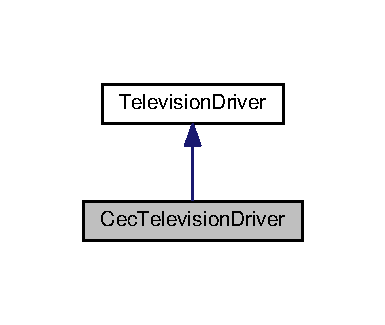
\includegraphics[width=185pt]{classCecTelevisionDriver__inherit__graph}
\end{center}
\end{figure}


Collaboration diagram for Cec\+Television\+Driver\+:
\nopagebreak
\begin{figure}[H]
\begin{center}
\leavevmode
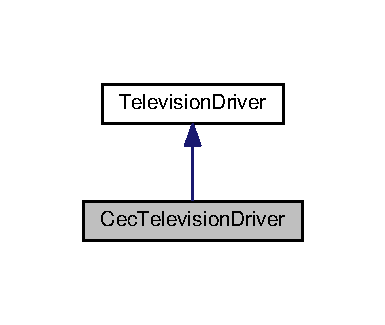
\includegraphics[width=185pt]{classCecTelevisionDriver__coll__graph}
\end{center}
\end{figure}
\subsection*{Public Member Functions}
\begin{DoxyCompactItemize}
\item 
\hyperlink{classCecTelevisionDriver_a6fc32515ca7c7dc05e8256c1b5dc15ca}{Cec\+Television\+Driver} ()
\item 
\hyperlink{classCecTelevisionDriver_a5d21757c126ad25a5d45686ba76f487a}{$\sim$\+Cec\+Television\+Driver} ()
\item 
const \hyperlink{structTelevisionStatus}{Television\+Status} \& \hyperlink{classCecTelevisionDriver_a7951a3e9f71c699b880af51a12a1764d}{get\+\_\+video\+\_\+status} () const 
\item 
void \hyperlink{classCecTelevisionDriver_a57d6f70f16b35e54e6ce3423c96f0c18}{power\+\_\+on} ()
\item 
void \hyperlink{classCecTelevisionDriver_a5ef7d248edd310444f670499ccf8f765}{power\+\_\+off} ()
\end{DoxyCompactItemize}


\subsection{Detailed Description}
This is an adapter used to handle a television through H\+D\+M\+I cable. This use the Lib\+C\+E\+C to perform operations. 

\subsection{Constructor \& Destructor Documentation}
\hypertarget{classCecTelevisionDriver_a6fc32515ca7c7dc05e8256c1b5dc15ca}{\index{Cec\+Television\+Driver@{Cec\+Television\+Driver}!Cec\+Television\+Driver@{Cec\+Television\+Driver}}
\index{Cec\+Television\+Driver@{Cec\+Television\+Driver}!Cec\+Television\+Driver@{Cec\+Television\+Driver}}
\subsubsection[{Cec\+Television\+Driver}]{\setlength{\rightskip}{0pt plus 5cm}Cec\+Television\+Driver\+::\+Cec\+Television\+Driver (
\begin{DoxyParamCaption}
{}
\end{DoxyParamCaption}
)}}\label{classCecTelevisionDriver_a6fc32515ca7c7dc05e8256c1b5dc15ca}
Default constructor. Initialize each data and television's connection. \hypertarget{classCecTelevisionDriver_a5d21757c126ad25a5d45686ba76f487a}{\index{Cec\+Television\+Driver@{Cec\+Television\+Driver}!````~Cec\+Television\+Driver@{$\sim$\+Cec\+Television\+Driver}}
\index{````~Cec\+Television\+Driver@{$\sim$\+Cec\+Television\+Driver}!Cec\+Television\+Driver@{Cec\+Television\+Driver}}
\subsubsection[{$\sim$\+Cec\+Television\+Driver}]{\setlength{\rightskip}{0pt plus 5cm}Cec\+Television\+Driver\+::$\sim$\+Cec\+Television\+Driver (
\begin{DoxyParamCaption}
{}
\end{DoxyParamCaption}
)}}\label{classCecTelevisionDriver_a5d21757c126ad25a5d45686ba76f487a}
Default destructor. It release used resources. 

\subsection{Member Function Documentation}
\hypertarget{classCecTelevisionDriver_a7951a3e9f71c699b880af51a12a1764d}{\index{Cec\+Television\+Driver@{Cec\+Television\+Driver}!get\+\_\+video\+\_\+status@{get\+\_\+video\+\_\+status}}
\index{get\+\_\+video\+\_\+status@{get\+\_\+video\+\_\+status}!Cec\+Television\+Driver@{Cec\+Television\+Driver}}
\subsubsection[{get\+\_\+video\+\_\+status}]{\setlength{\rightskip}{0pt plus 5cm}const {\bf Television\+Status}\& Cec\+Television\+Driver\+::get\+\_\+video\+\_\+status (
\begin{DoxyParamCaption}
{}
\end{DoxyParamCaption}
) const\hspace{0.3cm}{\ttfamily [virtual]}}}\label{classCecTelevisionDriver_a7951a3e9f71c699b880af51a12a1764d}
This method gets the current status of the video. \begin{DoxyReturn}{Returns}
A struct that describe the status of teh video.
\end{DoxyReturn}
== C\+O\+N\+T\+R\+A\+C\+T == \begin{DoxyPrecond}{Precondition}
No preconditions. 
\end{DoxyPrecond}
\begin{DoxyPostcond}{Postcondition}
Returned pointer is not N\+U\+L\+L.
\end{DoxyPostcond}
 

Implements \hyperlink{classTelevisionDriver_a5dcdc6c2b9c8bab8471080a44ac19f8e}{Television\+Driver}.

\hypertarget{classCecTelevisionDriver_a5ef7d248edd310444f670499ccf8f765}{\index{Cec\+Television\+Driver@{Cec\+Television\+Driver}!power\+\_\+off@{power\+\_\+off}}
\index{power\+\_\+off@{power\+\_\+off}!Cec\+Television\+Driver@{Cec\+Television\+Driver}}
\subsubsection[{power\+\_\+off}]{\setlength{\rightskip}{0pt plus 5cm}void Cec\+Television\+Driver\+::power\+\_\+off (
\begin{DoxyParamCaption}
{}
\end{DoxyParamCaption}
)\hspace{0.3cm}{\ttfamily [virtual]}}}\label{classCecTelevisionDriver_a5ef7d248edd310444f670499ccf8f765}
Power off the television. It must be called if the television is powered on.

== C\+O\+N\+T\+R\+A\+C\+T == \begin{DoxyPrecond}{Precondition}
Video must be powered on. See get\+\_\+video\+\_\+status. 
\end{DoxyPrecond}
\begin{DoxyPostcond}{Postcondition}
Video is powered off, its power\+\_\+status is off.
\end{DoxyPostcond}
 

Implements \hyperlink{classTelevisionDriver_a91298bc5e5c89b2fe2d125f84e111b09}{Television\+Driver}.

\hypertarget{classCecTelevisionDriver_a57d6f70f16b35e54e6ce3423c96f0c18}{\index{Cec\+Television\+Driver@{Cec\+Television\+Driver}!power\+\_\+on@{power\+\_\+on}}
\index{power\+\_\+on@{power\+\_\+on}!Cec\+Television\+Driver@{Cec\+Television\+Driver}}
\subsubsection[{power\+\_\+on}]{\setlength{\rightskip}{0pt plus 5cm}void Cec\+Television\+Driver\+::power\+\_\+on (
\begin{DoxyParamCaption}
{}
\end{DoxyParamCaption}
)\hspace{0.3cm}{\ttfamily [virtual]}}}\label{classCecTelevisionDriver_a57d6f70f16b35e54e6ce3423c96f0c18}
Power on the television. It must be called if the television is powered off.

== C\+O\+N\+T\+R\+A\+C\+T == \begin{DoxyPrecond}{Precondition}
Video must be powered off. See get\+\_\+video\+\_\+status. 
\end{DoxyPrecond}
\begin{DoxyPostcond}{Postcondition}
Video is powered on, its power\+\_\+status is on.
\end{DoxyPostcond}
 

Implements \hyperlink{classTelevisionDriver_a24163794dbfdf4273425b8b13cae0676}{Television\+Driver}.



The documentation for this class was generated from the following file\+:\begin{DoxyCompactItemize}
\item 
include/tv\+\_\+driver/\hyperlink{cec__television__driver_8hh}{cec\+\_\+television\+\_\+driver.\+hh}\end{DoxyCompactItemize}

\hypertarget{classTelevisionDriver}{\section{Television\+Driver Class Reference}
\label{classTelevisionDriver}\index{Television\+Driver@{Television\+Driver}}
}


{\ttfamily \#include $<$television\+\_\+driver.\+hh$>$}



Inheritance diagram for Television\+Driver\+:
\nopagebreak
\begin{figure}[H]
\begin{center}
\leavevmode
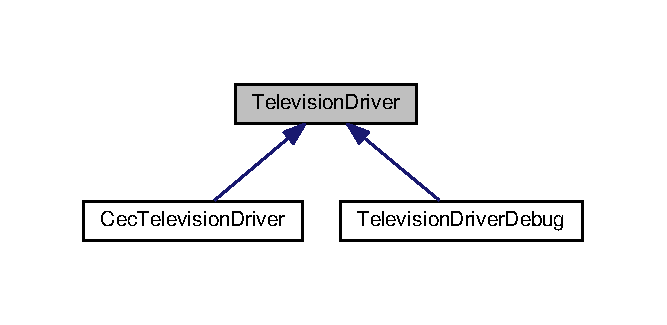
\includegraphics[width=320pt]{classTelevisionDriver__inherit__graph}
\end{center}
\end{figure}
\subsection*{Public Member Functions}
\begin{DoxyCompactItemize}
\item 
\hyperlink{classTelevisionDriver_ac0af9a24e93a01169ac6d3e3f7863802}{Television\+Driver} ()
\item 
virtual \hyperlink{classTelevisionDriver_addb7dec34cf34b135dc9da2ae68e2fe6}{$\sim$\+Television\+Driver} ()
\item 
virtual const \hyperlink{structTelevisionStatus}{Television\+Status} \& \hyperlink{classTelevisionDriver_a5dcdc6c2b9c8bab8471080a44ac19f8e}{get\+\_\+video\+\_\+status} () const =0
\item 
virtual void \hyperlink{classTelevisionDriver_a24163794dbfdf4273425b8b13cae0676}{power\+\_\+on} ()=0
\item 
virtual void \hyperlink{classTelevisionDriver_a91298bc5e5c89b2fe2d125f84e111b09}{power\+\_\+off} ()=0
\end{DoxyCompactItemize}


\subsection{Detailed Description}
This class is an abstract class used to represent a generic video. It is a wrapper for libraries used to handle with theme. 

\subsection{Constructor \& Destructor Documentation}
\hypertarget{classTelevisionDriver_ac0af9a24e93a01169ac6d3e3f7863802}{\index{Television\+Driver@{Television\+Driver}!Television\+Driver@{Television\+Driver}}
\index{Television\+Driver@{Television\+Driver}!Television\+Driver@{Television\+Driver}}
\subsubsection[{Television\+Driver}]{\setlength{\rightskip}{0pt plus 5cm}Television\+Driver\+::\+Television\+Driver (
\begin{DoxyParamCaption}
{}
\end{DoxyParamCaption}
)}}\label{classTelevisionDriver_ac0af9a24e93a01169ac6d3e3f7863802}
Default constructor. \hypertarget{classTelevisionDriver_addb7dec34cf34b135dc9da2ae68e2fe6}{\index{Television\+Driver@{Television\+Driver}!````~Television\+Driver@{$\sim$\+Television\+Driver}}
\index{````~Television\+Driver@{$\sim$\+Television\+Driver}!Television\+Driver@{Television\+Driver}}
\subsubsection[{$\sim$\+Television\+Driver}]{\setlength{\rightskip}{0pt plus 5cm}virtual Television\+Driver\+::$\sim$\+Television\+Driver (
\begin{DoxyParamCaption}
{}
\end{DoxyParamCaption}
)\hspace{0.3cm}{\ttfamily [virtual]}}}\label{classTelevisionDriver_addb7dec34cf34b135dc9da2ae68e2fe6}
Virtual Destructor 

\subsection{Member Function Documentation}
\hypertarget{classTelevisionDriver_a5dcdc6c2b9c8bab8471080a44ac19f8e}{\index{Television\+Driver@{Television\+Driver}!get\+\_\+video\+\_\+status@{get\+\_\+video\+\_\+status}}
\index{get\+\_\+video\+\_\+status@{get\+\_\+video\+\_\+status}!Television\+Driver@{Television\+Driver}}
\subsubsection[{get\+\_\+video\+\_\+status}]{\setlength{\rightskip}{0pt plus 5cm}virtual const {\bf Television\+Status}\& Television\+Driver\+::get\+\_\+video\+\_\+status (
\begin{DoxyParamCaption}
{}
\end{DoxyParamCaption}
) const\hspace{0.3cm}{\ttfamily [pure virtual]}}}\label{classTelevisionDriver_a5dcdc6c2b9c8bab8471080a44ac19f8e}
This method gets the current status of the video. \begin{DoxyReturn}{Returns}
A struct that describe the status of teh video.
\end{DoxyReturn}
== C\+O\+N\+T\+R\+A\+C\+T == \begin{DoxyPrecond}{Precondition}
No preconditions. 
\end{DoxyPrecond}
\begin{DoxyPostcond}{Postcondition}
Returned pointer is not N\+U\+L\+L. 
\end{DoxyPostcond}


Implemented in \hyperlink{classTelevisionDriverDebug_ad23820f9639351e2b222fdb941ee2792}{Television\+Driver\+Debug}, and \hyperlink{classCecTelevisionDriver_a7951a3e9f71c699b880af51a12a1764d}{Cec\+Television\+Driver}.

\hypertarget{classTelevisionDriver_a91298bc5e5c89b2fe2d125f84e111b09}{\index{Television\+Driver@{Television\+Driver}!power\+\_\+off@{power\+\_\+off}}
\index{power\+\_\+off@{power\+\_\+off}!Television\+Driver@{Television\+Driver}}
\subsubsection[{power\+\_\+off}]{\setlength{\rightskip}{0pt plus 5cm}virtual void Television\+Driver\+::power\+\_\+off (
\begin{DoxyParamCaption}
{}
\end{DoxyParamCaption}
)\hspace{0.3cm}{\ttfamily [pure virtual]}}}\label{classTelevisionDriver_a91298bc5e5c89b2fe2d125f84e111b09}
Power off the television. It must be called if the television is powered on.

== C\+O\+N\+T\+R\+A\+C\+T == \begin{DoxyPrecond}{Precondition}
Video must be powered on. See get\+\_\+video\+\_\+status. 
\end{DoxyPrecond}
\begin{DoxyPostcond}{Postcondition}
Video is powered off, its power\+\_\+status is off. 
\end{DoxyPostcond}


Implemented in \hyperlink{classTelevisionDriverDebug_aae9ffd499fa9b050e4eadb846b0b7257}{Television\+Driver\+Debug}, and \hyperlink{classCecTelevisionDriver_a5ef7d248edd310444f670499ccf8f765}{Cec\+Television\+Driver}.

\hypertarget{classTelevisionDriver_a24163794dbfdf4273425b8b13cae0676}{\index{Television\+Driver@{Television\+Driver}!power\+\_\+on@{power\+\_\+on}}
\index{power\+\_\+on@{power\+\_\+on}!Television\+Driver@{Television\+Driver}}
\subsubsection[{power\+\_\+on}]{\setlength{\rightskip}{0pt plus 5cm}virtual void Television\+Driver\+::power\+\_\+on (
\begin{DoxyParamCaption}
{}
\end{DoxyParamCaption}
)\hspace{0.3cm}{\ttfamily [pure virtual]}}}\label{classTelevisionDriver_a24163794dbfdf4273425b8b13cae0676}
Power on the television. It must be called if the television is powered off.

== C\+O\+N\+T\+R\+A\+C\+T == \begin{DoxyPrecond}{Precondition}
Video must be powered off. See get\+\_\+video\+\_\+status. 
\end{DoxyPrecond}
\begin{DoxyPostcond}{Postcondition}
Video is powered on, its power\+\_\+status is on. 
\end{DoxyPostcond}


Implemented in \hyperlink{classTelevisionDriverDebug_a1f5e16575b48f979a44d81fba14a836e}{Television\+Driver\+Debug}, and \hyperlink{classCecTelevisionDriver_a57d6f70f16b35e54e6ce3423c96f0c18}{Cec\+Television\+Driver}.



The documentation for this class was generated from the following file\+:\begin{DoxyCompactItemize}
\item 
include/tv\+\_\+driver/\hyperlink{television__driver_8hh}{television\+\_\+driver.\+hh}\end{DoxyCompactItemize}

\hypertarget{classTelevisionDriverDebug}{\section{Television\+Driver\+Debug Class Reference}
\label{classTelevisionDriverDebug}\index{Television\+Driver\+Debug@{Television\+Driver\+Debug}}
}


{\ttfamily \#include $<$television\+\_\+driver\+\_\+debug.\+hh$>$}



Inheritance diagram for Television\+Driver\+Debug\+:
\nopagebreak
\begin{figure}[H]
\begin{center}
\leavevmode
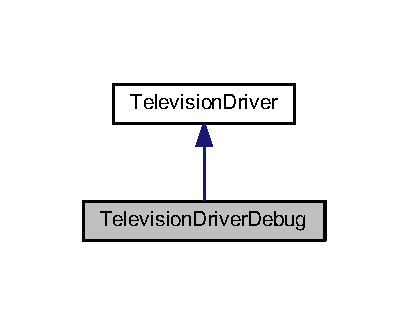
\includegraphics[width=196pt]{classTelevisionDriverDebug__inherit__graph}
\end{center}
\end{figure}


Collaboration diagram for Television\+Driver\+Debug\+:
\nopagebreak
\begin{figure}[H]
\begin{center}
\leavevmode
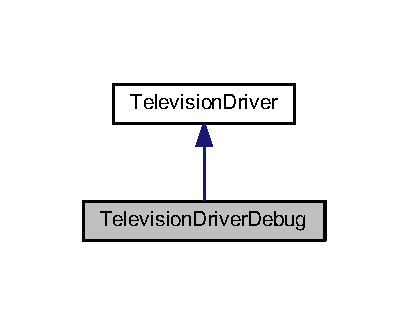
\includegraphics[width=196pt]{classTelevisionDriverDebug__coll__graph}
\end{center}
\end{figure}
\subsection*{Public Member Functions}
\begin{DoxyCompactItemize}
\item 
\hyperlink{classTelevisionDriverDebug_a6519c487afc26a2fdb9869a9733705fa}{Television\+Driver\+Debug} (std\+::unique\+\_\+ptr$<$ \hyperlink{classTelevisionDriver}{Television\+Driver} $>$ television\+\_\+driver)
\item 
\hyperlink{classTelevisionDriverDebug_afd370254cfa8eae311fb85752a385c72}{$\sim$\+Television\+Driver\+Debug} ()
\item 
const \hyperlink{structTelevisionStatus}{Television\+Status} \& \hyperlink{classTelevisionDriverDebug_ad23820f9639351e2b222fdb941ee2792}{get\+\_\+video\+\_\+status} () const 
\item 
void \hyperlink{classTelevisionDriverDebug_a1f5e16575b48f979a44d81fba14a836e}{power\+\_\+on} ()
\item 
void \hyperlink{classTelevisionDriverDebug_aae9ffd499fa9b050e4eadb846b0b7257}{power\+\_\+off} ()
\end{DoxyCompactItemize}


\subsection{Detailed Description}
This television driver is used for debug purpose. It take an other driver, like proxy pattern, to perform the core operations. This is used to make assertion on pre conditions before each operations and post condition after execution of each methods. See Television\+Adapter documentation to know the Contracts to be checked.~\newline
 N\+O\+T\+E\+: The proxied object is taken as unique\+\_\+ptr and the ownership is moved to this object through std\+::move function. 

\subsection{Constructor \& Destructor Documentation}
\hypertarget{classTelevisionDriverDebug_a6519c487afc26a2fdb9869a9733705fa}{\index{Television\+Driver\+Debug@{Television\+Driver\+Debug}!Television\+Driver\+Debug@{Television\+Driver\+Debug}}
\index{Television\+Driver\+Debug@{Television\+Driver\+Debug}!Television\+Driver\+Debug@{Television\+Driver\+Debug}}
\subsubsection[{Television\+Driver\+Debug}]{\setlength{\rightskip}{0pt plus 5cm}Television\+Driver\+Debug\+::\+Television\+Driver\+Debug (
\begin{DoxyParamCaption}
\item[{std\+::unique\+\_\+ptr$<$ {\bf Television\+Driver} $>$}]{television\+\_\+driver}
\end{DoxyParamCaption}
)\hspace{0.3cm}{\ttfamily [explicit]}}}\label{classTelevisionDriverDebug_a6519c487afc26a2fdb9869a9733705fa}
Constructor with one parameter. It initialize this adapter using the one passed as parameter to have a proxy pattern behavior.~\newline
 I\+M\+P\+O\+R\+T\+A\+N\+T\+: It is passed as unique\+\_\+ptr and ownership is moved to this object throug std\+::move function. 
\begin{DoxyParams}{Parameters}
{\em television\+\_\+driver} & -\/ Smart pointer to the driver. It must be not null. \\
\hline
\end{DoxyParams}
\hypertarget{classTelevisionDriverDebug_afd370254cfa8eae311fb85752a385c72}{\index{Television\+Driver\+Debug@{Television\+Driver\+Debug}!````~Television\+Driver\+Debug@{$\sim$\+Television\+Driver\+Debug}}
\index{````~Television\+Driver\+Debug@{$\sim$\+Television\+Driver\+Debug}!Television\+Driver\+Debug@{Television\+Driver\+Debug}}
\subsubsection[{$\sim$\+Television\+Driver\+Debug}]{\setlength{\rightskip}{0pt plus 5cm}Television\+Driver\+Debug\+::$\sim$\+Television\+Driver\+Debug (
\begin{DoxyParamCaption}
{}
\end{DoxyParamCaption}
)}}\label{classTelevisionDriverDebug_afd370254cfa8eae311fb85752a385c72}
Default destructor. 

\subsection{Member Function Documentation}
\hypertarget{classTelevisionDriverDebug_ad23820f9639351e2b222fdb941ee2792}{\index{Television\+Driver\+Debug@{Television\+Driver\+Debug}!get\+\_\+video\+\_\+status@{get\+\_\+video\+\_\+status}}
\index{get\+\_\+video\+\_\+status@{get\+\_\+video\+\_\+status}!Television\+Driver\+Debug@{Television\+Driver\+Debug}}
\subsubsection[{get\+\_\+video\+\_\+status}]{\setlength{\rightskip}{0pt plus 5cm}const {\bf Television\+Status}\& Television\+Driver\+Debug\+::get\+\_\+video\+\_\+status (
\begin{DoxyParamCaption}
{}
\end{DoxyParamCaption}
) const\hspace{0.3cm}{\ttfamily [virtual]}}}\label{classTelevisionDriverDebug_ad23820f9639351e2b222fdb941ee2792}
This method gets the current status of the video. \begin{DoxyReturn}{Returns}
A struct that describe the status of teh video.
\end{DoxyReturn}
== C\+O\+N\+T\+R\+A\+C\+T == \begin{DoxyPrecond}{Precondition}
No preconditions. 
\end{DoxyPrecond}
\begin{DoxyPostcond}{Postcondition}
Returned pointer is not N\+U\+L\+L.
\end{DoxyPostcond}
 

Implements \hyperlink{classTelevisionDriver_a5dcdc6c2b9c8bab8471080a44ac19f8e}{Television\+Driver}.

\hypertarget{classTelevisionDriverDebug_aae9ffd499fa9b050e4eadb846b0b7257}{\index{Television\+Driver\+Debug@{Television\+Driver\+Debug}!power\+\_\+off@{power\+\_\+off}}
\index{power\+\_\+off@{power\+\_\+off}!Television\+Driver\+Debug@{Television\+Driver\+Debug}}
\subsubsection[{power\+\_\+off}]{\setlength{\rightskip}{0pt plus 5cm}void Television\+Driver\+Debug\+::power\+\_\+off (
\begin{DoxyParamCaption}
{}
\end{DoxyParamCaption}
)\hspace{0.3cm}{\ttfamily [virtual]}}}\label{classTelevisionDriverDebug_aae9ffd499fa9b050e4eadb846b0b7257}
Power off the television. It must be called if the television is powered on.

== C\+O\+N\+T\+R\+A\+C\+T == \begin{DoxyPrecond}{Precondition}
Video must be powered on. See get\+\_\+video\+\_\+status. 
\end{DoxyPrecond}
\begin{DoxyPostcond}{Postcondition}
Video is powered off, its power\+\_\+status is off.
\end{DoxyPostcond}
 

Implements \hyperlink{classTelevisionDriver_a91298bc5e5c89b2fe2d125f84e111b09}{Television\+Driver}.

\hypertarget{classTelevisionDriverDebug_a1f5e16575b48f979a44d81fba14a836e}{\index{Television\+Driver\+Debug@{Television\+Driver\+Debug}!power\+\_\+on@{power\+\_\+on}}
\index{power\+\_\+on@{power\+\_\+on}!Television\+Driver\+Debug@{Television\+Driver\+Debug}}
\subsubsection[{power\+\_\+on}]{\setlength{\rightskip}{0pt plus 5cm}void Television\+Driver\+Debug\+::power\+\_\+on (
\begin{DoxyParamCaption}
{}
\end{DoxyParamCaption}
)\hspace{0.3cm}{\ttfamily [virtual]}}}\label{classTelevisionDriverDebug_a1f5e16575b48f979a44d81fba14a836e}
Power on the television. It must be called if the television is powered off.

== C\+O\+N\+T\+R\+A\+C\+T == \begin{DoxyPrecond}{Precondition}
Video must be powered off. See get\+\_\+video\+\_\+status. 
\end{DoxyPrecond}
\begin{DoxyPostcond}{Postcondition}
Video is powered on, its power\+\_\+status is on.
\end{DoxyPostcond}
 

Implements \hyperlink{classTelevisionDriver_a24163794dbfdf4273425b8b13cae0676}{Television\+Driver}.



The documentation for this class was generated from the following file\+:\begin{DoxyCompactItemize}
\item 
include/tv\+\_\+driver/\hyperlink{television__driver__debug_8hh}{television\+\_\+driver\+\_\+debug.\+hh}\end{DoxyCompactItemize}

\hypertarget{structTelevisionStatus}{\section{Television\+Status Struct Reference}
\label{structTelevisionStatus}\index{Television\+Status@{Television\+Status}}
}


Status of the television. This struct is used to store the informations of the video's status.  




{\ttfamily \#include $<$television\+\_\+status.\+hh$>$}

\subsection*{Public Member Functions}
\begin{DoxyCompactItemize}
\item 
\hyperlink{structTelevisionStatus_adde5868b55df0547cfcc772a7c82af3e}{Television\+Status} ()
\item 
\hyperlink{structTelevisionStatus_a29fc37e00c26001339422e7eb3e7f449}{$\sim$\+Television\+Status} ()
\end{DoxyCompactItemize}
\subsection*{Public Attributes}
\begin{DoxyCompactItemize}
\item 
\hyperlink{television__status_8hh_a65e6bb4d942c22dba9975253b0a1d73f}{Power\+Status} \hyperlink{structTelevisionStatus_a900ca63a3edb937ec4312ff11ea09ea1}{power\+\_\+status}
\end{DoxyCompactItemize}


\subsection{Detailed Description}
Status of the television. This struct is used to store the informations of the video's status. 

\subsection{Constructor \& Destructor Documentation}
\hypertarget{structTelevisionStatus_adde5868b55df0547cfcc772a7c82af3e}{\index{Television\+Status@{Television\+Status}!Television\+Status@{Television\+Status}}
\index{Television\+Status@{Television\+Status}!Television\+Status@{Television\+Status}}
\subsubsection[{Television\+Status}]{\setlength{\rightskip}{0pt plus 5cm}Television\+Status\+::\+Television\+Status (
\begin{DoxyParamCaption}
{}
\end{DoxyParamCaption}
)}}\label{structTelevisionStatus_adde5868b55df0547cfcc772a7c82af3e}
Default constructor. \hypertarget{structTelevisionStatus_a29fc37e00c26001339422e7eb3e7f449}{\index{Television\+Status@{Television\+Status}!````~Television\+Status@{$\sim$\+Television\+Status}}
\index{````~Television\+Status@{$\sim$\+Television\+Status}!Television\+Status@{Television\+Status}}
\subsubsection[{$\sim$\+Television\+Status}]{\setlength{\rightskip}{0pt plus 5cm}Television\+Status\+::$\sim$\+Television\+Status (
\begin{DoxyParamCaption}
{}
\end{DoxyParamCaption}
)}}\label{structTelevisionStatus_a29fc37e00c26001339422e7eb3e7f449}
Default destructor. 

\subsection{Member Data Documentation}
\hypertarget{structTelevisionStatus_a900ca63a3edb937ec4312ff11ea09ea1}{\index{Television\+Status@{Television\+Status}!power\+\_\+status@{power\+\_\+status}}
\index{power\+\_\+status@{power\+\_\+status}!Television\+Status@{Television\+Status}}
\subsubsection[{power\+\_\+status}]{\setlength{\rightskip}{0pt plus 5cm}{\bf Power\+Status} Television\+Status\+::power\+\_\+status}}\label{structTelevisionStatus_a900ca63a3edb937ec4312ff11ea09ea1}
This is the current power status of the video. It is used to check if it is on or off. 

The documentation for this struct was generated from the following file\+:\begin{DoxyCompactItemize}
\item 
include/tv\+\_\+driver/\hyperlink{television__status_8hh}{television\+\_\+status.\+hh}\end{DoxyCompactItemize}

\chapter{File Documentation}
\hypertarget{driver__factory_8hh}{\section{include/driver\+\_\+factory.hh File Reference}
\label{driver__factory_8hh}\index{include/driver\+\_\+factory.\+hh@{include/driver\+\_\+factory.\+hh}}
}


This file contains the factory function used to create the television driver.  


{\ttfamily \#include \char`\"{}./tv\+\_\+driver/television\+\_\+driver.\+hh\char`\"{}}\\*
Include dependency graph for driver\+\_\+factory.\+hh\+:
\nopagebreak
\begin{figure}[H]
\begin{center}
\leavevmode
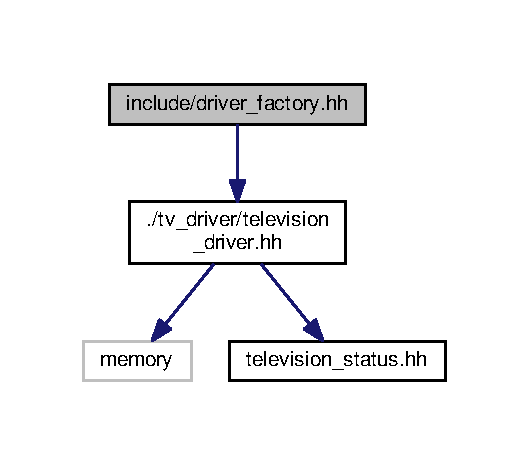
\includegraphics[width=254pt]{driver__factory_8hh__incl}
\end{center}
\end{figure}
\subsection*{Macros}
\begin{DoxyCompactItemize}
\item 
\hypertarget{driver__factory_8hh_a3960ae721ce97d89c42f711cf2b1f2a2}{\#define {\bfseries D\+R\+I\+V\+E\+R\+\_\+\+F\+A\+C\+T\+O\+R\+Y\+\_\+\+I\+N\+C\+L\+U\+D\+E\+\_\+\+G\+U\+A\+R\+D}~1}\label{driver__factory_8hh_a3960ae721ce97d89c42f711cf2b1f2a2}

\end{DoxyCompactItemize}
\subsection*{Functions}
\begin{DoxyCompactItemize}
\item 
\hyperlink{classTelevisionDriver}{Television\+Driver} $\ast$ \hyperlink{driver__factory_8hh_a87ec6e595e8230b584446fdff67b0db2}{create\+\_\+television\+\_\+driver} ()
\end{DoxyCompactItemize}


\subsection{Detailed Description}
This file contains the factory function used to create the television driver. 



\subsection{Function Documentation}
\hypertarget{driver__factory_8hh_a87ec6e595e8230b584446fdff67b0db2}{\index{driver\+\_\+factory.\+hh@{driver\+\_\+factory.\+hh}!create\+\_\+television\+\_\+driver@{create\+\_\+television\+\_\+driver}}
\index{create\+\_\+television\+\_\+driver@{create\+\_\+television\+\_\+driver}!driver\+\_\+factory.\+hh@{driver\+\_\+factory.\+hh}}
\subsubsection[{create\+\_\+television\+\_\+driver}]{\setlength{\rightskip}{0pt plus 5cm}{\bf Television\+Driver}$\ast$ create\+\_\+television\+\_\+driver (
\begin{DoxyParamCaption}
{}
\end{DoxyParamCaption}
)}}\label{driver__factory_8hh_a87ec6e595e8230b584446fdff67b0db2}
Create a an instance of television driver according to the compiler flag\+: release or debug version according to N\+D\+E\+B\+U\+G flag.~\newline
 It implements a singleton pattern, so if it called twice, both pointers points to the same object. \begin{DoxyReturn}{Returns}
A pointer to the television driver. ~\newline
 I\+M\+P\+O\+R\+T\+A\+N\+T\+: The ownership is satic scope so the requestor must not matter of driver destruction. 
\end{DoxyReturn}

\hypertarget{cec__television__connection_8hh}{\section{include/tv\+\_\+driver/cec\+\_\+television\+\_\+connection.hh File Reference}
\label{cec__television__connection_8hh}\index{include/tv\+\_\+driver/cec\+\_\+television\+\_\+connection.\+hh@{include/tv\+\_\+driver/cec\+\_\+television\+\_\+connection.\+hh}}
}


This file contains the definition of the connection object used to check status of the cec device and connect it when it is not connected.  


{\ttfamily \#include $<$libcec/cec.\+h$>$}\\*
Include dependency graph for cec\+\_\+television\+\_\+connection.\+hh\+:
\nopagebreak
\begin{figure}[H]
\begin{center}
\leavevmode
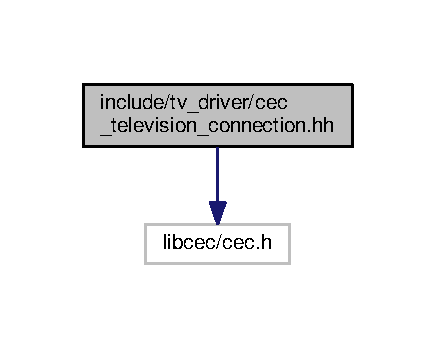
\includegraphics[width=209pt]{cec__television__connection_8hh__incl}
\end{center}
\end{figure}
This graph shows which files directly or indirectly include this file\+:
\nopagebreak
\begin{figure}[H]
\begin{center}
\leavevmode
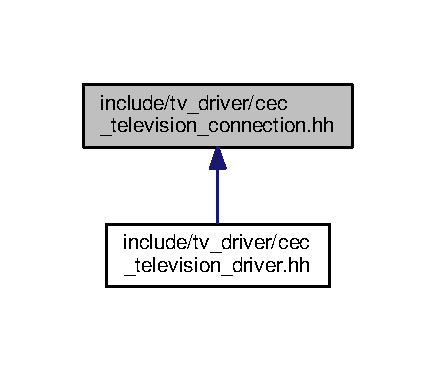
\includegraphics[width=209pt]{cec__television__connection_8hh__dep__incl}
\end{center}
\end{figure}
\subsection*{Classes}
\begin{DoxyCompactItemize}
\item 
class \hyperlink{classCecTelevisionConnection}{Cec\+Television\+Connection}
\end{DoxyCompactItemize}


\subsection{Detailed Description}
This file contains the definition of the connection object used to check status of the cec device and connect it when it is not connected. 


\hypertarget{cec__television__driver_8hh}{\section{include/tv\+\_\+driver/cec\+\_\+television\+\_\+driver.hh File Reference}
\label{cec__television__driver_8hh}\index{include/tv\+\_\+driver/cec\+\_\+television\+\_\+driver.\+hh@{include/tv\+\_\+driver/cec\+\_\+television\+\_\+driver.\+hh}}
}


This file contains the television driver implemented through the libcec.  


{\ttfamily \#include $<$memory$>$}\\*
{\ttfamily \#include $<$libcec/cec.\+h$>$}\\*
{\ttfamily \#include \char`\"{}television\+\_\+driver.\+hh\char`\"{}}\\*
{\ttfamily \#include \char`\"{}television\+\_\+status.\+hh\char`\"{}}\\*
{\ttfamily \#include \char`\"{}cec\+\_\+television\+\_\+connection.\+hh\char`\"{}}\\*
Include dependency graph for cec\+\_\+television\+\_\+driver.\+hh\+:
\nopagebreak
\begin{figure}[H]
\begin{center}
\leavevmode
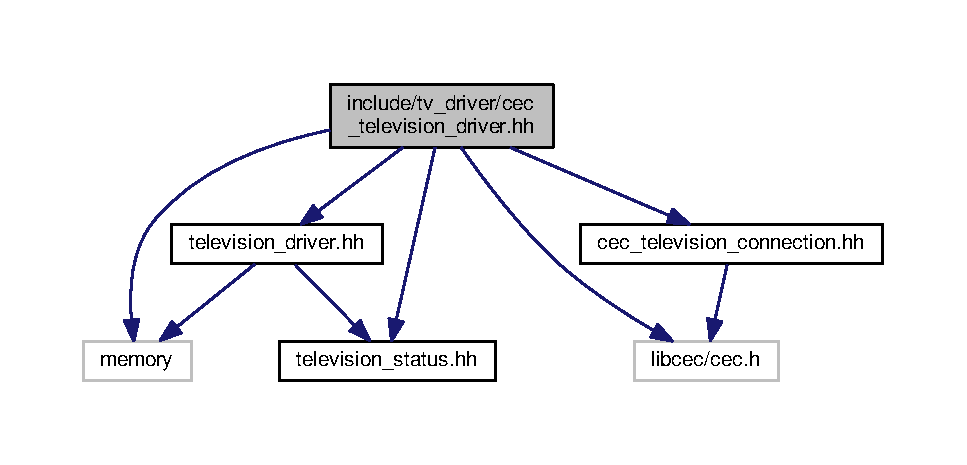
\includegraphics[width=350pt]{cec__television__driver_8hh__incl}
\end{center}
\end{figure}
\subsection*{Classes}
\begin{DoxyCompactItemize}
\item 
class \hyperlink{classCecTelevisionDriver}{Cec\+Television\+Driver}
\end{DoxyCompactItemize}
\subsection*{Macros}
\begin{DoxyCompactItemize}
\item 
\hypertarget{cec__television__driver_8hh_aafe39fbbaeed9bc4cd833e5bfe530309}{\#define {\bfseries C\+E\+C\+\_\+\+T\+E\+L\+E\+V\+I\+S\+I\+O\+N\+\_\+\+D\+R\+I\+V\+E\+R\+\_\+\+I\+N\+C\+L\+U\+D\+E\+\_\+\+G\+U\+A\+R\+D}~1}\label{cec__television__driver_8hh_aafe39fbbaeed9bc4cd833e5bfe530309}

\end{DoxyCompactItemize}


\subsection{Detailed Description}
This file contains the television driver implemented through the libcec. 


\hypertarget{television__driver_8hh}{\section{include/tv\+\_\+driver/television\+\_\+driver.hh File Reference}
\label{television__driver_8hh}\index{include/tv\+\_\+driver/television\+\_\+driver.\+hh@{include/tv\+\_\+driver/television\+\_\+driver.\+hh}}
}


This file contains the defintion of the television driver class used to perform operation on tv. This is an abstract class.  


{\ttfamily \#include $<$memory$>$}\\*
{\ttfamily \#include \char`\"{}television\+\_\+status.\+hh\char`\"{}}\\*
Include dependency graph for television\+\_\+driver.\+hh\+:
\nopagebreak
\begin{figure}[H]
\begin{center}
\leavevmode
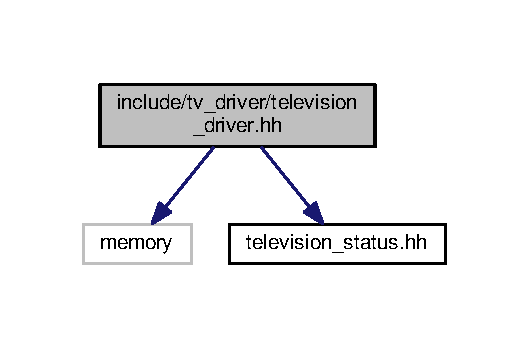
\includegraphics[width=254pt]{television__driver_8hh__incl}
\end{center}
\end{figure}
This graph shows which files directly or indirectly include this file\+:
\nopagebreak
\begin{figure}[H]
\begin{center}
\leavevmode
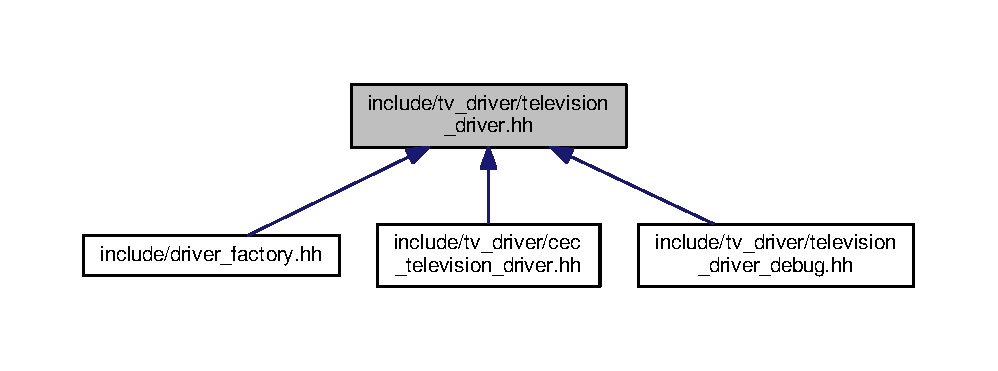
\includegraphics[width=350pt]{television__driver_8hh__dep__incl}
\end{center}
\end{figure}
\subsection*{Classes}
\begin{DoxyCompactItemize}
\item 
class \hyperlink{classTelevisionDriver}{Television\+Driver}
\end{DoxyCompactItemize}


\subsection{Detailed Description}
This file contains the defintion of the television driver class used to perform operation on tv. This is an abstract class. 


\hypertarget{television__driver__debug_8hh}{\section{include/tv\+\_\+driver/television\+\_\+driver\+\_\+debug.hh File Reference}
\label{television__driver__debug_8hh}\index{include/tv\+\_\+driver/television\+\_\+driver\+\_\+debug.\+hh@{include/tv\+\_\+driver/television\+\_\+driver\+\_\+debug.\+hh}}
}


This file contains the definition of the television driver used for debug purpose. It implements a proxy pattern to check assertions of proxied object.  


{\ttfamily \#include $<$memory$>$}\\*
{\ttfamily \#include \char`\"{}television\+\_\+status.\+hh\char`\"{}}\\*
{\ttfamily \#include \char`\"{}television\+\_\+driver.\+hh\char`\"{}}\\*
Include dependency graph for television\+\_\+driver\+\_\+debug.\+hh\+:
\nopagebreak
\begin{figure}[H]
\begin{center}
\leavevmode
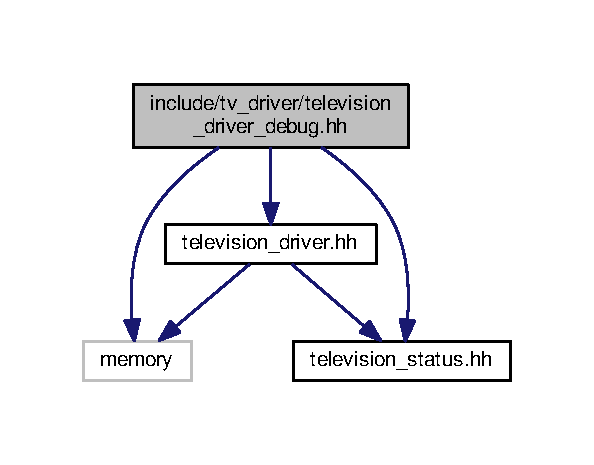
\includegraphics[width=285pt]{television__driver__debug_8hh__incl}
\end{center}
\end{figure}
\subsection*{Classes}
\begin{DoxyCompactItemize}
\item 
class \hyperlink{classTelevisionDriverDebug}{Television\+Driver\+Debug}
\end{DoxyCompactItemize}


\subsection{Detailed Description}
This file contains the definition of the television driver used for debug purpose. It implements a proxy pattern to check assertions of proxied object. 


\hypertarget{television__status_8hh}{\section{include/tv\+\_\+driver/television\+\_\+status.hh File Reference}
\label{television__status_8hh}\index{include/tv\+\_\+driver/television\+\_\+status.\+hh@{include/tv\+\_\+driver/television\+\_\+status.\+hh}}
}


This file contains the struct used to represent the status of the telvision.  


This graph shows which files directly or indirectly include this file\+:
\nopagebreak
\begin{figure}[H]
\begin{center}
\leavevmode
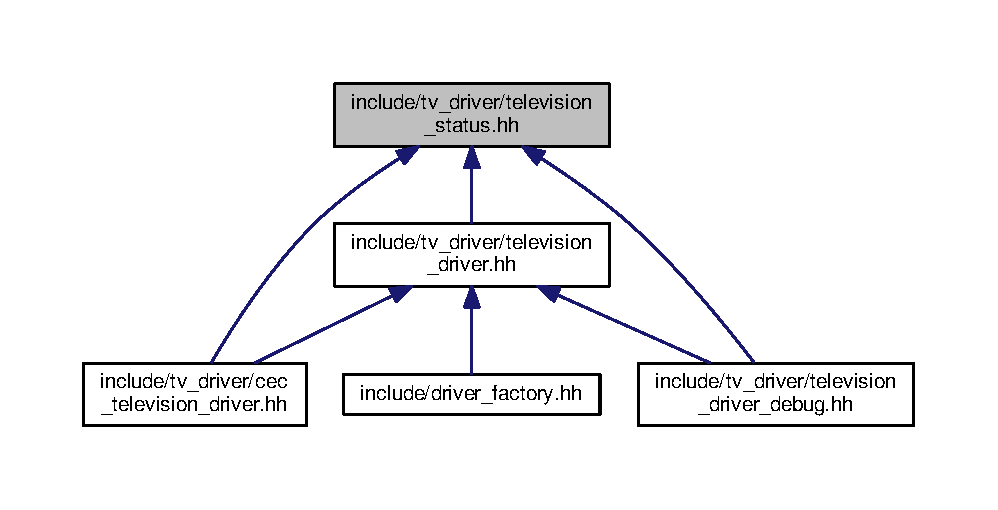
\includegraphics[width=350pt]{television__status_8hh__dep__incl}
\end{center}
\end{figure}
\subsection*{Classes}
\begin{DoxyCompactItemize}
\item 
struct \hyperlink{structTelevisionStatus}{Television\+Status}
\begin{DoxyCompactList}\small\item\em Status of the television. This struct is used to store the informations of the video's status. \end{DoxyCompactList}\end{DoxyCompactItemize}
\subsection*{Enumerations}
\begin{DoxyCompactItemize}
\item 
enum \hyperlink{television__status_8hh_a65e6bb4d942c22dba9975253b0a1d73f}{Power\+Status} \{ \hyperlink{television__status_8hh_a65e6bb4d942c22dba9975253b0a1d73fa53ace14c115e45153a1c9105accceb4c}{off} = 0, 
\hyperlink{television__status_8hh_a65e6bb4d942c22dba9975253b0a1d73faf3be4933da71233c5904ec919ac1fdb0}{on} = 1
 \}
\end{DoxyCompactItemize}


\subsection{Detailed Description}
This file contains the struct used to represent the status of the telvision. 



\subsection{Enumeration Type Documentation}
\hypertarget{television__status_8hh_a65e6bb4d942c22dba9975253b0a1d73f}{\index{television\+\_\+status.\+hh@{television\+\_\+status.\+hh}!Power\+Status@{Power\+Status}}
\index{Power\+Status@{Power\+Status}!television\+\_\+status.\+hh@{television\+\_\+status.\+hh}}
\subsubsection[{Power\+Status}]{\setlength{\rightskip}{0pt plus 5cm}enum {\bf Power\+Status}}}\label{television__status_8hh_a65e6bb4d942c22dba9975253b0a1d73f}
This is an enumeration type used to represent the status of the video's power\+: on or off. \begin{Desc}
\item[Enumerator]\par
\begin{description}
\index{off@{off}!television\+\_\+status.\+hh@{television\+\_\+status.\+hh}}\index{television\+\_\+status.\+hh@{television\+\_\+status.\+hh}!off@{off}}\item[{\em 
\hypertarget{television__status_8hh_a65e6bb4d942c22dba9975253b0a1d73fa53ace14c115e45153a1c9105accceb4c}{off}\label{television__status_8hh_a65e6bb4d942c22dba9975253b0a1d73fa53ace14c115e45153a1c9105accceb4c}
}]Video is off or in stand by. \index{on@{on}!television\+\_\+status.\+hh@{television\+\_\+status.\+hh}}\index{television\+\_\+status.\+hh@{television\+\_\+status.\+hh}!on@{on}}\item[{\em 
\hypertarget{television__status_8hh_a65e6bb4d942c22dba9975253b0a1d73faf3be4933da71233c5904ec919ac1fdb0}{on}\label{television__status_8hh_a65e6bb4d942c22dba9975253b0a1d73faf3be4933da71233c5904ec919ac1fdb0}
}]Video is on or is powering on. \end{description}
\end{Desc}

%--- End generated contents ---

% Index
\newpage
\phantomsection
\addcontentsline{toc}{chapter}{Index}
\printindex

\end{document}
